% -*- latex -*-
%%%%%%%%%%%%%%%%%%%%%%%%%%%%%%%%%%%%%%%%%%%%%%%%%%%%%%%%%%%%%%%%
%%%%
%%%% This TeX file is part of the course
%%%% Introduction to Scientific Programming in C++/Fortran2003
%%%% copyright 2017-2020 Victor Eijkhout eijkhout@tacc.utexas.edu
%%%%
%%%% struct.tex : about structures
%%%%
%%%%%%%%%%%%%%%%%%%%%%%%%%%%%%%%%%%%%%%%%%%%%%%%%%%%%%%%%%%%%%%%

\Level 0 {Why structures?}
\label{sec:struct}

You have seen the basic datatypes in section~\ref{sec:ctypes}. These
are enough to program whatever you want, but it would be nice if the
language had some datatypes that are more abstract, closer to the
terms in which you think about your application. For instance, if you
are programming something to do with geometry, you had rather talk
about points than explicitly having to manipulate their coordinates.

Structures are a
first way to define your own datatypes\footnote
{Note for instructors: structures in C++ are actually largely the same
  as classes. This chapter really teaches structures as they
  appear in~C. However, that's a good first step towards classes.}
A~\indexcdef{struct}
acts like a datatype for which you choose the name. A~\lstinline$struct$
contains other datatypes; these can be elementary, or other structs.
%
\verbatimsnippet{structdef}

The elements of a structure are also called
\emph{members}\index{member!of struct}.
  
\begin{slide}{Bundling information}
  \label{sl:struct-why}
  Sometimes a number of variables belong logically together. For
  instance two doubles can be the $x,y$ components of a point.

  This can be captured in the \lstinline$struct$ construct.

  \verbatimsnippet{structdef}

  (This is a type definition; it can go in the main program or before it.)

The elements of a structure are usually called \indexterm{members}.
\end{slide}

The reason for using structures is to `raise the level of
abstraction': instead of talking about \lstinline{x,y}-values, you can
now talk about points and such. This makes your code look closer to
the application you are modeling.

\Level 0 {The basics of structures}

A structure behaves like a data type: you declare variables of the
structure type, and you use them in your program. The new aspect is
that you first need to define the structure type. This definition can
be done inside your main program or before it. The latter is
preferable.

\begin{lstlisting}
// definition of the struct
struct StructName { int num; double val; }
int main() {
  // declaration of struct variables
  StructName mystruct1,mystruct2;
  .... code that uses your structures ....
}
\end{lstlisting}

\begin{slide}{How to use structures}
  \label{sl:structinprog}
  \begin{enumerate}
  \item Define the structure: what members are in it.
  \item Declare some structure variables;
  \item Use these variables.
  \end{enumerate}
\begin{lstlisting}
// definition of the struct
struct StructName { int num; double val; }
int main() {
  // declaration of struct variables
  StructName mystruct1,mystruct2;
  .... code that uses your structures ....
}
\end{lstlisting}
\end{slide}

There are various ways of setting the members of the structure:
\begin{itemize}
\item You can set defaults that hold for any structure of that type;
\item you can all members at once;
\item or you can set any member individually.
\end{itemize}

\begin{block}{Struct initialization}
  \label{sl:structinit}
  You assign a whole struct, or set defaults in the definition.
  %
  \verbatimsnippet{pointinit}
\end{block}

\begin{block}{Using structures}
  \label{sl:struct-use}
  Once you have defined a structure, you can make variables of that
  type. Setting and initializing them takes a new syntax:
  %
  \snippetwithoutput{structuse}{struct}{point}
  %
  Period syntax: compare to possessive `apostrophe-s' in English.
\end{block}

\begin{review}
  \label{rev:struct-def}
  True or false?

  \footnotesize
  \begin{itemize}
  \item All members of a struct have to be of the same type.
    \slackpollTF+struct members all the same type+
  \item Writing
\begin{lstlisting}
struct numbered { int n; double x; };
\end{lstlisting}
creates a structure with an integer and a double as members.
\slackpollTF+'struct numbered { int n; double x; };' creates struct with int and double+
\item All members of a struct have to be of different types.
  \slackpollTF+All struct members have to be different types+
\item With the above definition and \lstinline$struct numbered xn;$,
\begin{lstlisting}
cout << xn << endl;
\end{lstlisting}
Is this correct C++?
\slackpollTF+'cout << xn << endl;' legal?+
\item With the same definitions, is this correct C++?
\begin{lstlisting}
xn.x = xn.n+1;
\end{lstlisting}
\slackpollTF-'xn.x = xn.n+1;' legal?-
  \end{itemize}
\end{review}

\begin{exercise}
  \label{ex:gridstruct}
  Define a struct \n{GridPoint} that models a grid point,
  meaning a point with integer coordinates.
  The \indexterm{Manhattan distance} is defined
  as the sum of (absolute values of) the components.
  Read the values of the two components, and
  if the $x$ component is more than the $y$,
  print `this location is cross-town',
  otherwise print `this location is uptown'.
  \skeleton{gridpoint}
\end{exercise}

\begin{remark}
  Before \cppstandard{14},
  if you used initializations in the \lstinline$struct$ definition,
  you could not use the brace-assignment. This has been fixed.
  %
  \verbatimsnippet{pointinit14}
\end{remark}

\Level 0 {Structures and functions}

You can use structures with functions, just as you could with
elementary datatypes.

\begin{block}{Functions on structures}
  \label{sl:struct-pass}
  You can pass a structure to a function:

  \footnotesize
  \snippetwithoutput{structpass}{struct}{pointfun}
\end{block}

\begin{exercise}
  \label{ex:vecstruct-angle}
  \hbox{%
    \begin{minipage}[t]{.6\hsize}
      Write a point structure, and a function that, given such a  point, returns the
      angle with the $x$-axis. (Hint: the \lstinline$atan$ function is in \lstinline$cmath$)
    \end{minipage}
    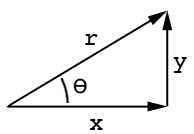
\includegraphics[scale=.4]{xy-atan}
    }

  \answerwithoutput{anglepi4}{struct}{pointangle}
\end{exercise}

The mechanisms of \indextermbus{parameter}{passing by value} and
\indextermbus{parameter}{passing by reference} apply to structures just as
to simple datatypes.

\begin{exercise}
  \label{ex:vecstruct-flip}
  Write a \lstinline$void$ function that has a \lstinline$struct Point$ parameter,
  and exchanges its coordinates:
  \[ \begin{pmatrix}2.5\\3.5\end{pmatrix} \rightarrow
    \begin{pmatrix}3.5\\2.5\end{pmatrix} \]
  \answerwithoutput{flip32}{struct}{pointflip}
\end{exercise}

\begin{exercise}
  \label{ex:vecstruct-scale}
  Write a function $y=f(x,a)$ that takes a \lstinline$struct Point$ and
  \lstinline$double$ parameter as input, and returns a point that is the
  input multiplied by the scalar.
  \[ \begin{pmatrix}2.5\\3.5\end{pmatrix},3 \rightarrow
    \begin{pmatrix}7.5\\10.5\end{pmatrix} \]
\end{exercise}

\begin{comment}
  \begin{exercise}
    \label{ex:primestruct}
    If you are doing the prime project (chapter~\ref{ch:prime}) you can
    now do exercise~\ref{ex:prime:struct}.
  \end{exercise}
\end{comment}

\begin{exercise}
  \label{ex:vecstruct}
  Write a function \lstinline$inner_product$ that takes two \lstinline$Point$
  structures and computes the inner product. Test your code on some points where
  you know the answer.
\end{exercise}

For a more sophisticated version of this exercise:

\begin{exercise}
  \label{ex:vecortho}
  Write two functions:
  \begin{enumerate}
  \item \lstinline{rotate} takes a point~$v$ and a scalar~$\alpha$
    and returns a point that is $v$~rotated over~$\alpha$.
  \item \lstinline$inner_product$ that takes two points and returns
    their inner product.
  \end{enumerate}
  Now apply the inner product function on a point~$v$ and $v$~rotated
  by $\pi/2$. Is their inner product zero?

  Here you can learn about floating point arithmetic and floating point error.

  Now write a boolean function \lstinline{is_orthogonal}
  that works in the presence of floating point error.
\end{exercise}

\begin{block}{Denotations}
  \label{sl:struct-denote}
  You can use \indextermbus{initializer}{list}s as struct
  \emph{denotations}\index{struct!denotation}\\
  (with the \lstinline{distance} function previous defined):
  %
  \snippetwithoutput[pointfun]{structdenote}{struct}{pointdenote}
  %\snippetwithoutput{structdenote}{struct}{pointdenote}
\end{block}

\begin{exercise}
  \label{ex:struct-denote}
  Take exercise \ref{ex:vecstruct} and rewrite it to use denotations.
\end{exercise}

\begin{block}{Returning structures}
  \label{sl:struct-return}
  You can return a structure from a function:
  %
  \snippetwithoutput{structreturn}{struct}{pointadd}

  (In case you're wondering about scopes and lifetimes here: the
  explanation is that the returned value is copied.)
\end{block}

\begin{exercise}
  \label{ex:matstruct}
  Write a $2\times 2$ matrix class (that is, a structure storing 4
  real numbers), and write a function \lstinline$multiply$
  that multiplies a matrix times a vector.

  Can you make a matrix structure that is based on the vector
  structure
  (essentially the same as a \lstinline{Point} struct),
  for instance using vectors to store the matrix rows, and
  then using the inner product method to multiply matrices?
\end{exercise}

